% Sample paper for testing Paper Companion. The paper and its authors are fictional.
\documentclass[conference,letterpaper]{IEEEtran}
\input{glyphtounicode}
\pdfgentounicode=1
\usepackage[T1]{fontenc}
\usepackage{newtxtext,newtxmath}
\usepackage{booktabs}
\usepackage{pgfplots}
\pgfplotsset{compat=1.18}
\usepgfplotslibrary{colormaps}
\usetikzlibrary{arrows.meta,positioning}
\usepackage[hidelinks]{hyperref}
\hypersetup{pdftitle={Sparse Routing Attention: Scaling Transformers to Long Documents Without Quadratic Cost},pdfauthor={Maya R. Okafor, Daniel Lindqvist, Priya Raman}}

\definecolor{sra}{RGB}{31,78,156}
\definecolor{dense}{RGB}{192,57,43}

\begin{document}

\title{Sparse Routing Attention: Scaling Transformers to\\Long Documents Without Quadratic Cost}

\author{\IEEEauthorblockN{Maya R. Okafor\IEEEauthorrefmark{1}, Daniel Lindqvist\IEEEauthorrefmark{1}, and Priya Raman\IEEEauthorrefmark{2}}
\IEEEauthorblockA{\IEEEauthorrefmark{1}Department of Computer Science, Northfield University\qquad
\IEEEauthorrefmark{2}Halden Institute for Machine Learning}}

\maketitle

\begin{abstract}
Transformer models excel at document understanding, but the quadratic cost of self-attention limits how much text they can process in a single pass. Existing remedies, such as sliding windows and low-rank projections, reduce cost at the expense of long-range reasoning. We propose Sparse Routing Attention (SRA), a mechanism in which each token is routed to a small, learned set of memory slots that summarize distant context. Routing is trained end to end with a load-balancing objective and adds less than 2\% to the parameter count. On four long-document benchmarks, SRA matches dense attention at 4K tokens and outperforms it beyond 16K, while using 6.3$\times$ less memory at 32K tokens. We further show that the learned routes align with document structure, sending tokens to slots associated with sections, tables, and citations.
\end{abstract}

\begin{IEEEkeywords}
transformers, sparse attention, long-context modeling, document understanding, efficient inference.
\end{IEEEkeywords}

\section{Introduction}

Long documents such as legal contracts, scientific articles, and technical manuals often run to tens of thousands of tokens. Answering a question about such a document frequently requires combining evidence that appears far apart: a definition in the opening section, a table in the appendix, and a qualifying remark buried in a footnote. Standard transformers [1] attend from every token to every other token, so their compute and memory grow quadratically with sequence length. In practice this caps the usable context at a few thousand tokens on commodity accelerators.

A large body of work has sought to relax this limit. Local and sliding-window attention [2], [3] restricts each token to a fixed neighborhood, which is efficient but blind to distant evidence. Global-token schemes [4] add a handful of tokens that attend everywhere, yet the choice of which tokens become global is fixed in advance. Low-rank and kernel approximations [5], [6] compress the attention matrix but tend to blur the fine-grained interactions that matter for extraction tasks. Retrieval-augmented approaches [7] sidestep the problem by fetching relevant passages, at the cost of a separate index and a non-differentiable lookup step.

\begin{figure}[t]
\centering
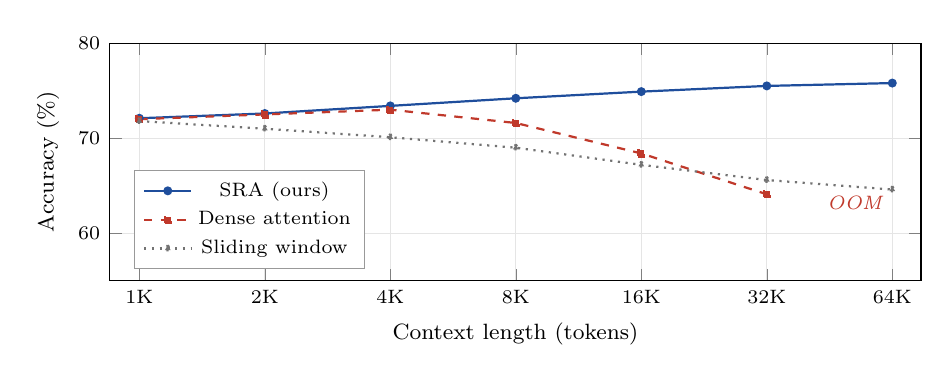
\begin{tikzpicture}
\begin{axis}[
  width=0.98\columnwidth, height=4.6cm,
  xmode=log, log basis x=2,
  xtick={1,2,4,8,16,32,64}, xticklabels={1K,2K,4K,8K,16K,32K,64K},
  xmin=0.85, xmax=75, ymin=55, ymax=80,
  xlabel={Context length (tokens)}, ylabel={Accuracy (\%)},
  label style={font=\footnotesize}, tick label style={font=\scriptsize},
  legend style={font=\scriptsize, at={(0.03,0.05)}, anchor=south west, draw=black!40},
  grid=major, grid style={black!10}]
\addplot[sra, thick, mark=*, mark size=1.2pt] coordinates {(1,72.1)(2,72.6)(4,73.4)(8,74.2)(16,74.9)(32,75.5)(64,75.8)};
\addlegendentry{SRA (ours)}
\addplot[dense, thick, dashed, mark=square*, mark size=1.1pt] coordinates {(1,72.0)(2,72.5)(4,73.0)(8,71.6)(16,68.4)(32,64.1)};
\addlegendentry{Dense attention}
\addplot[black!55, dotted, thick, mark=triangle*, mark size=1.2pt] coordinates {(1,71.8)(2,71.0)(4,70.1)(8,69.0)(16,67.2)(32,65.6)(64,64.6)};
\addlegendentry{Sliding window}
\node[dense, font=\scriptsize\itshape] at (axis cs:52,63.2) {OOM};
\end{axis}
\end{tikzpicture}
\caption{Question-answering accuracy versus context length, averaged over four long-document benchmarks. Dense attention exhausts memory beyond 32K tokens on a single 80 GB accelerator, while SRA continues to improve.}
\label{fig:accuracy}
\end{figure}

We argue that the right question is not how to approximate full attention, but where each token needs to look. Most tokens in a long document depend on a small number of distant regions, and those regions are largely predictable from local content. A token inside a results table, for instance, almost always needs the column headers and the method description, and rarely needs the acknowledgments.

Building on this observation, we introduce Sparse Routing Attention (SRA). SRA maintains a bank of $k$ memory slots, each of which aggregates a learned subset of the sequence. Every token attends densely to its local window and sparsely to the top-$r$ slots chosen by a lightweight router. Because $k$ and $r$ are small constants, the cost of the global pathway grows linearly with length. The router is trained jointly with the model using a load-balancing loss that keeps slot usage even and prevents collapse onto a few popular slots.

Our contributions are as follows:
\begin{itemize}
\item We propose SRA, a drop-in replacement for self-attention whose global cost is linear in sequence length.
\item We show that SRA matches dense attention at short lengths and surpasses it beyond 16K tokens on four benchmarks.
\item We analyze the learned routes and find that they recover section and table structure without supervision.
\end{itemize}

The remainder of this paper is organized as follows. Section II reviews related work. Section III describes the routing mechanism and its training objective. Section IV presents experiments on four long-document benchmarks, and Section V discusses limitations and future work.

\section{Related Work}

\textit{Efficient attention.} Early efforts to scale attention fixed a sparsity pattern ahead of time, combining strided and local patterns so that information can propagate across the sequence in a few layers [2]. Later models mixed local windows with a small set of global tokens [4] or replaced the softmax kernel with a random-feature approximation [6]. These methods are efficient but treat every input the same way, regardless of its structure.

\textit{Learned sparsity.} A second line of work learns which positions to attend to. Hashing-based methods group similar queries and keys into buckets [8], and clustering approaches assign tokens to centroids that are updated during training [9]. Our router is closest in spirit to these methods, but it routes to persistent memory slots rather than to other tokens, which keeps the routing decision cheap and stable across layers.

\textit{Memory-augmented models.} Recurrent memory and compressive caches carry a summary of earlier segments forward as the model reads [10]. These summaries are written in order and read by every token alike. SRA instead lets each token choose which summaries to read, so a token in a table and a token in the introduction can draw on entirely different parts of the document.

\section{Method}

\begin{figure}[t]
\centering
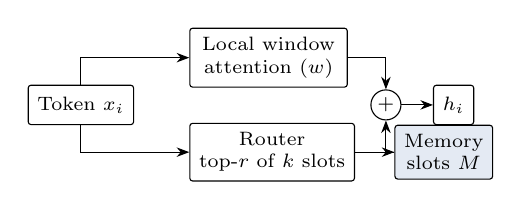
\begin{tikzpicture}[font=\scriptsize, box/.style={draw, rounded corners=1pt, minimum height=5mm, align=center}]
\node[box, minimum width=12mm] (x) {Token $x_i$};
\node[box, right=7mm of x, yshift=6mm, minimum width=20mm] (loc) {Local window\\attention ($w$)};
\node[box, right=7mm of x, yshift=-6mm, minimum width=20mm] (rout) {Router\\top-$r$ of $k$ slots};
\node[box, right=5mm of rout, minimum width=12mm, fill=sra!12] (mem) {Memory\\slots $M$};
\node[draw, circle, inner sep=1pt, right=30mm of x] (sum) {$+$};
\node[box, right=4mm of sum] (h) {$h_i$};
\draw[-{Stealth[length=1.6mm]}] (x) |- (loc);
\draw[-{Stealth[length=1.6mm]}] (x) |- (rout);
\draw[-{Stealth[length=1.6mm]}] (rout) -- (mem);
\draw[-{Stealth[length=1.6mm]}] (loc) -| (sum);
\draw[-{Stealth[length=1.6mm]}] (mem) -| (sum);
\draw[-{Stealth[length=1.6mm]}] (sum) -- (h);
\end{tikzpicture}
\caption{Overview of Sparse Routing Attention. Each token attends densely to its local window and sparsely to the top-$r$ memory slots chosen by the router. The two pathways are summed before the output projection.}
\label{fig:overview}
\end{figure}

SRA replaces each self-attention layer with two pathways that run side by side: a local pathway that sees nearby tokens exactly, and a global pathway that sees the whole document through a few learned summaries. The final hidden state of each token therefore combines a precise view of its neighborhood with a coarse but global view of the document. We describe each component in turn.

\subsection{Local Window Attention}

Given an input sequence $X = (x_1, \ldots, x_n)$, each token attends to the $w$ tokens on either side of it using standard scaled dot-product attention. We use $w = 256$ in all experiments, which keeps the local pathway inexpensive while covering most sentence- and paragraph-level dependencies.
\begin{equation}
a_i = \mathrm{softmax}\!\left(q_i K_{(i)}^{\top} / \sqrt{d}\right) V_{(i)}
\end{equation}

\subsection{Routing to Memory Slots}

The global pathway maintains $k$ memory slots $M = (m_1, \ldots, m_k)$. Each slot is computed as a weighted average of token representations, where the weights come from a learned assignment matrix. A router scores every slot for every token and keeps the $r$ highest-scoring slots; all other scores are set to zero. In practice we use $k = 64$ and $r = 4$, so each token reads from only four summaries regardless of document length.
\begin{equation}
g_i = \mathrm{top}\text{-}r\left(\mathrm{softmax}(W_r x_i)\right)
\end{equation}
The token then attends over its selected slots, and the result is added to the output of the local pathway. Because routing scores are computed from the token itself, the cost of this step is linear in $n$.
\begin{equation}
h_i = a_i + \textstyle\sum_j g_{ij} \cdot \mathrm{Attn}(x_i, m_j)
\end{equation}

\subsection{Load Balancing}

Without regularization, the router quickly learns to send most tokens to a handful of slots, leaving the rest unused. Following prior work on mixture-of-experts models, we add an auxiliary loss that penalizes the squared coefficient of variation of slot usage within each batch. The loss weight is set to 0.01 and is annealed to 0.001 over the first 10K steps.

We found that this simple objective was sufficient to keep more than 95\% of slots active throughout training. Removing it reduced average accuracy by 3.1 points and caused two of the four benchmarks to diverge.

\subsection{Complexity}

The local pathway costs $O(nw)$ and the global pathway $O(nk + nrd)$, giving an overall cost that is linear in $n$ for fixed $w$, $k$, and $r$. At 32K tokens this reduces peak activation memory from 61 GB to 9.7 GB relative to dense attention with the same hidden size and number of layers.

\subsection{Implementation Details}

We implement SRA as a fused kernel that computes local attention, router scores, and slot attention in a single pass over the sequence. The top-$r$ selection is performed with a partial sort on the accelerator, and slot summaries are recomputed every layer from the current hidden states.

\section{Experimental Setup}

\textit{Benchmarks.} We evaluate on four long-document tasks: question answering over scientific articles, clause extraction from contracts, multi-hop reasoning over technical manuals, and summarization of government reports. Median document lengths range from 9K to 41K tokens.

\textit{Baselines.} We compare against dense attention, a sliding-window model, a global-token model, a kernel approximation, and a retrieval-augmented pipeline. All models share the same tokenizer, hidden size of 1024, and 24 layers, and are trained on the same 120B-token corpus.

\textit{Training.} Models are trained for 200K steps with a batch size of 256 sequences and a cosine learning-rate schedule peaking at $3 \times 10^{-4}$. Sequence length is increased from 4K to 32K tokens over the first half of training.

\textit{Evaluation.} We report exact-match accuracy for question answering, F1 for clause extraction, and ROUGE-L for summarization. Each result is the mean of three runs with different random seeds; standard deviations are below 0.4 points in all cases and are omitted for space. Documents longer than the evaluated context length are truncated from the end.

\begin{table*}[t]
\centering
\caption{Results on four long-document benchmarks. Best results in bold.}
\label{tab:results}
\begin{tabular}{lcccccc}
\toprule
Model & SciQA & Contracts & ManualHop & GovSum & Avg. & Mem. (GB) \\
\midrule
Dense attention & 71.4 & 63.8 & 48.2 & 34.1 & 54.4 & 61.0 \\
Sliding window & 68.9 & 60.2 & 41.7 & 32.6 & 50.9 & 8.1 \\
Global tokens & 70.2 & 62.5 & 45.9 & 33.4 & 53.0 & 10.4 \\
Kernel approx. & 67.5 & 59.1 & 43.0 & 31.8 & 50.4 & 7.6 \\
Retrieval pipeline & 70.8 & 64.1 & 47.3 & 32.9 & 53.8 & 12.2 \\
\midrule
SRA (ours) & \textbf{73.6} & \textbf{66.2} & \textbf{52.9} & \textbf{35.0} & \textbf{56.9} & 9.7 \\
\bottomrule
\end{tabular}
\end{table*}

\section{Results}

\subsection{Main Results}

Table I reports results on all four benchmarks. SRA achieves the best score on every task and improves the average by 2.5 points over dense attention, while using 6.3$\times$ less peak memory. The largest gain appears on ManualHop, where answers require combining evidence from sections that are often more than 20K tokens apart.

The sliding-window and kernel baselines are cheaper than dense attention but lose between 3.5 and 4.0 points on average. The retrieval pipeline is competitive on Contracts, where answers are usually contained in a single clause, but trails on tasks that require reasoning over several passages.

\subsection{Scaling With Context Length}

Fig. 1 shows how accuracy changes as more of each document is provided. Dense attention improves up to 4K tokens and then degrades, which we attribute to attention entropy rising as the number of candidate positions grows. SRA continues to improve up to 64K tokens, the longest length we tested.

\begin{figure}[t]
\centering
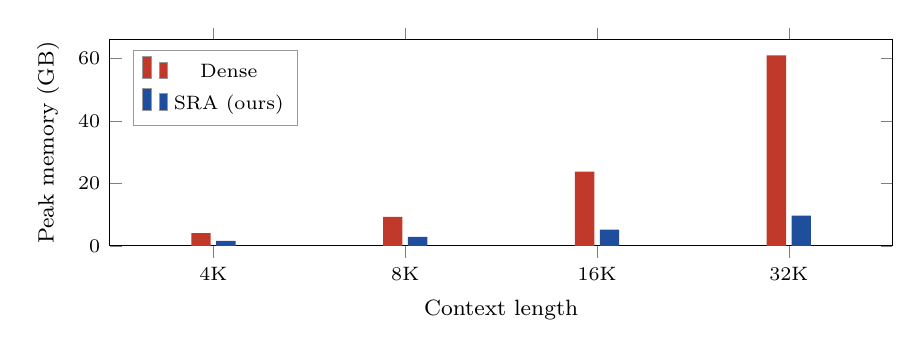
\begin{tikzpicture}
\begin{axis}[
  width=0.95\columnwidth, height=4.2cm, ybar, bar width=7pt,
  symbolic x coords={4K,8K,16K,32K}, xtick=data, ymin=0, ymax=66,
  xlabel={Context length}, ylabel={Peak memory (GB)},
  label style={font=\footnotesize}, tick label style={font=\scriptsize},
  legend style={font=\scriptsize, at={(0.03,0.95)}, anchor=north west, draw=black!40},
  enlarge x limits=0.18]
\addplot[fill=dense, draw=none] coordinates {(4K,4.1)(8K,9.3)(16K,23.8)(32K,61.0)};
\addlegendentry{Dense}
\addplot[fill=sra, draw=none] coordinates {(4K,1.6)(8K,2.9)(16K,5.2)(32K,9.7)};
\addlegendentry{SRA (ours)}
\end{axis}
\end{tikzpicture}
\caption{Peak activation memory during training for a single 24-layer model. Dense attention grows quadratically; SRA grows close to linearly.}
\label{fig:memory}
\end{figure}

\subsection{Efficiency}

Fig. 3 compares peak memory for dense attention and SRA. At 32K tokens SRA requires 9.7 GB, compared with 61 GB for dense attention. Throughput follows the same trend: SRA processes 2.8$\times$ more tokens per second at 16K and 5.1$\times$ more at 32K on the same hardware.

The overhead of routing is small. Computing router scores and selecting the top-$r$ slots accounts for 4.2\% of the forward pass at 32K tokens, and the load-balancing loss adds no measurable cost.

\subsection{Ablations}

We vary the number of slots $k$ and the number of selected slots $r$. Accuracy improves rapidly up to $k = 32$ and saturates around $k = 64$; increasing $r$ beyond 4 brings little benefit while raising cost. Replacing learned routing with a fixed assignment by position reduces the average score by 2.9 points, confirming that content-based routing is essential.

\section{Analysis}

\subsection{What Do the Routes Learn?}

To understand how the router uses its memory slots, we tag each token in 500 held-out scientific articles with the section it belongs to and record which slots it selects. Fig. 4 shows the resulting routing frequencies. Without any supervision, most slots specialize: tokens from the abstract and introduction share a pair of slots, method tokens use another, and tokens inside tables are routed almost exclusively to two dedicated slots.

This specialization explains much of the gain on ManualHop. When a question refers to a value in a table, tokens in the question are routed to the same slots as the table itself, giving the model a direct path to the evidence even when it lies tens of thousands of tokens away.

\begin{figure}[t]
\centering
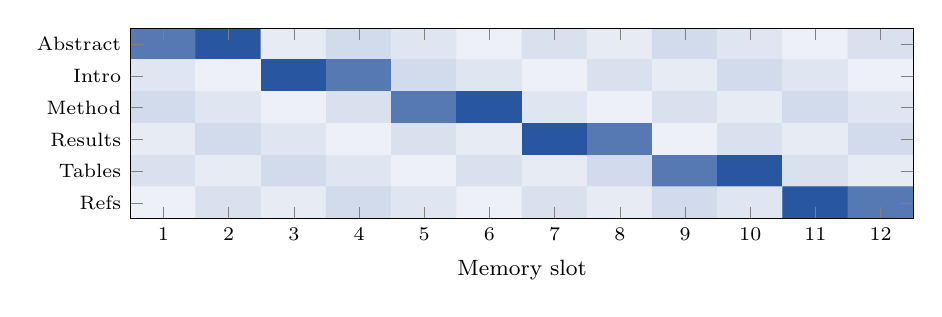
\begin{tikzpicture}
\begin{axis}[
  width=0.95\columnwidth, height=4.0cm,
  colormap={blues}{rgb255=(255,255,255) rgb255=(31,78,156)},
  point meta min=0, point meta max=1,
  xmin=0.5, xmax=12.5, ymin=0.5, ymax=6.5,
  xtick={1,...,12}, ytick={1,...,6},
  yticklabels={Refs,Tables,Results,Method,Intro,Abstract},
  xlabel={Memory slot}, label style={font=\footnotesize}, tick label style={font=\scriptsize},
  axis on top, enlargelimits=false]
\addplot[matrix plot*, mesh/cols=12, point meta=explicit] table[meta=c] {
x y c
1 6 0.75
2 6 0.95
3 6 0.11
4 6 0.20
5 6 0.14
6 6 0.08
7 6 0.17
8 6 0.11
9 6 0.20
10 6 0.14
11 6 0.08
12 6 0.17
1 5 0.14
2 5 0.08
3 5 0.95
4 5 0.75
5 5 0.20
6 5 0.14
7 5 0.08
8 5 0.17
9 5 0.11
10 5 0.20
11 5 0.14
12 5 0.08
1 4 0.20
2 4 0.14
3 4 0.08
4 4 0.17
5 4 0.75
6 4 0.95
7 4 0.14
8 4 0.08
9 4 0.17
10 4 0.11
11 4 0.20
12 4 0.14
1 3 0.11
2 3 0.20
3 3 0.14
4 3 0.08
5 3 0.17
6 3 0.11
7 3 0.95
8 3 0.75
9 3 0.08
10 3 0.17
11 3 0.11
12 3 0.20
1 2 0.17
2 2 0.11
3 2 0.20
4 2 0.14
5 2 0.08
6 2 0.17
7 2 0.11
8 2 0.20
9 2 0.75
10 2 0.95
11 2 0.17
12 2 0.11
1 1 0.08
2 1 0.17
3 1 0.11
4 1 0.20
5 1 0.14
6 1 0.08
7 1 0.17
8 1 0.11
9 1 0.20
10 1 0.14
11 1 0.95
12 1 0.75
};
\end{axis}
\end{tikzpicture}
\caption{Routing frequency between document sections and memory slots in layer 18, averaged over 500 held-out articles. Darker cells indicate that a slot is selected more often.}
\label{fig:routes}
\end{figure}

\subsection{Failure Cases}

We manually inspected 100 errors on SciQA. The most common failure, accounting for 38\% of errors, occurs when the answer depends on a number that appears only in a figure caption; caption tokens are routed inconsistently, likely because captions are short and scattered. A further 22\% of errors involve questions that require comparing more than three sections, which exceeds what four selected slots can easily summarize.

\section{Conclusion}

We introduced Sparse Routing Attention, which replaces the global component of self-attention with a small set of learned memory slots selected per token. SRA matches dense attention on short inputs, outperforms it on long ones, and uses a fraction of the memory. Its routes recover document structure without supervision, suggesting that much of what long-context models need from distant text can be captured by a few well-chosen summaries. Future work will explore routing across documents and adapting the number of slots to the input.

\begin{thebibliography}{10}
\bibitem{vaswani} A. Vaswani et al., ``Attention is all you need,'' in \textit{Proc. NeurIPS}, 2017.
\bibitem{child} R. Child, S. Gray, A. Radford, and I. Sutskever, ``Generating long sequences with sparse transformers,'' arXiv:1904.10509, 2019.
\bibitem{beltagy} I. Beltagy, M. E. Peters, and A. Cohan, ``Longformer: The long-document transformer,'' arXiv:2004.05150, 2020.
\bibitem{zaheer} M. Zaheer et al., ``Big Bird: Transformers for longer sequences,'' in \textit{Proc. NeurIPS}, 2020.
\bibitem{wang} S. Wang, B. Z. Li, M. Khabsa, H. Fang, and H. Ma, ``Linformer: Self-attention with linear complexity,'' arXiv:2006.04768, 2020.
\bibitem{choromanski} K. Choromanski et al., ``Rethinking attention with Performers,'' in \textit{Proc. ICLR}, 2021.
\bibitem{lewis} P. Lewis et al., ``Retrieval-augmented generation for knowledge-intensive NLP tasks,'' in \textit{Proc. NeurIPS}, 2020.
\bibitem{kitaev} N. Kitaev, {\L}. Kaiser, and A. Levskaya, ``Reformer: The efficient transformer,'' in \textit{Proc. ICLR}, 2020.
\bibitem{roy} A. Roy, M. Saffar, A. Vaswani, and D. Grangier, ``Efficient content-based sparse attention with routing transformers,'' \textit{TACL}, 2021.
\bibitem{rae} J. W. Rae, A. Potapenko, S. M. Jayakumar, and T. P. Lillicrap, ``Compressive transformers for long-range sequence modelling,'' in \textit{Proc. ICLR}, 2020.
\end{thebibliography}

\end{document}
